%%%%%%%%%%%%%%%%%%%%%%%%%%%%%%%%%%%%%%%%%
% Uppsala University Assignment Title Page 
% LaTeX Template
% Version 1.0 (27/12/12)
%
% This template has been downloaded from:
% http://www.LaTeXTemplates.com
%
% Original author:
% WikiBooks (http://en.wikibooks.org/wiki/LaTeX/Title_Creation)
% Modified by Elsa Slattegard to fit Uppsala university
% License:
% CC BY-NC-SA 3.0 (http://creativecommons.org/licenses/by-nc-sa/3.0/)

\title{LDSA Assignment A1}
%----------------------------------------------------------------------------------------
%	PACKAGES AND OTHER DOCUMENT CONFIGURATIONS
%----------------------------------------------------------------------------------------

\documentclass[12pt]{article}
\usepackage[english]{babel}
\usepackage[utf8x]{inputenc}
\usepackage{amsmath}
\usepackage{graphicx}
\usepackage{float}
\usepackage[colorinlistoftodos]{todonotes}

\begin{document}

\begin{titlepage}

\newcommand{\HRule}{\rule{\linewidth}{0.5mm}} % Defines a new command for the horizontal lines, change thickness here

\center % Center everything on the page
 
%----------------------------------------------------------------------------------------
%	HEADING SECTIONS
%----------------------------------------------------------------------------------------

\textsc{\LARGE Uppsala University}\\[1.5cm] % Name of your university/college
\includegraphics[scale=.1]{Uppsala_University_seal_svg.png}\\[1cm] % Include a department/university logo - this will require the graphicx package
\textsc{\Large Large Datasets For Scientific Applications}\\[0.5cm] % Major heading such as course name
\textsc{\large 1TD268}\\[0.5cm] % Minor heading such as course title

%----------------------------------------------------------------------------------------
%	TITLE SECTION
%----------------------------------------------------------------------------------------

\HRule \\[0.4cm]
{ \huge \bfseries Assignment A1}\\[0.4cm] % Title of your document
\HRule \\[1.5cm]
 
%----------------------------------------------------------------------------------------
%	AUTHOR SECTION
%----------------------------------------------------------------------------------------

\begin{minipage}{0.4\textwidth}
\begin{flushleft} \large
\emph{Author:}\\
Sudarsan \textsc{Bhargavan}\\ % Your name
\end{flushleft}

\end{minipage}\\[2cm]

% If you don't want a supervisor, uncomment the two lines below and remove the section above
%\Large \emph{Author:}\\
%John \textsc{Smith}\\[3cm] % Your name

%----------------------------------------------------------------------------------------
%	DATE SECTION
%----------------------------------------------------------------------------------------

{\large \today}\\[2cm] % Date, change the \today to a set date if you want to be precise

\vfill % Fill the rest of the page with whitespace

\end{titlepage}

\section{Introduction to Hadoop/HDFS WordCount}
\subsection{Questions}
\begin{enumerate}
\item Look at the contents of the folder “output” - what are the files place in there? What do they mean?
\newline
\newline
\textbf{Ans:}
\newline
	There are two files that are created when a job is completed successfully, viz;
    \begin{itemize}
    \item \textbf{\_SUCCESS}
    \item \textbf{part-r-00000}
    \end{itemize}
	The file named \_SUCCESS is needed when any application needs to check the completion of the result set by inspecting HDFS.
    
    The file named part-r-00000 contains the output of the map \& reduce jobs as the name has an \textbf{r} tag which signifies the type of the job and the \textbf{00000} signifies the number of the task. \cite{FIH}
\newline
\hrule
\item In this example we used Hadoop in “Local (Standalone) Mode”. What is the difference between this mode and the Pseudo-distributed mode?
\newline
\newline
\textbf{Ans:}
\newline
	\textbf{Local Standalone Mode:}
    \newline
    	In this mode hadoop is configured in a single node setup as a single java process, with no demons. Local file system is used instead of HDFS. There is a single data-node, single name-node and only one task-tracker.
    \newline
    \newline
    \textbf{Pseudo-Distributed Mode:}
    \newline
    	In this configuration hadoop is set to simulate a multi-node cluster in just one VM instance. Unlike local standalone mode, HDFS is used instead of the local file system, hadoop demons run on multiple JVM instances. \cite{MsIH}
\end{enumerate}
\hrule
\subsection{Questions}
\begin{enumerate}
\item What are the roles of the files core-site.xml and hdfs-site.xml ?
\newline
\newline
\textbf{Ans:}
\newline
	\textbf{core-site.xml:}
    \newline
    	The core-site.xml configuration file has \textbf{Hadoop's core} configurations. Such as the \textbf{core I/O settings}, port and IP configurations for the \textbf{NameNode daemon}.
    \newline
    \newline
    \textbf{hdfs-site.xml:}
    \newline
    	The hdfs-site.xml configuration file has (\textbf{Hdfs daemons}, \textbf{NameNode}, \textbf{SecondaryNameNode}, \textbf{DataNodes})'s configurations. Also \textbf{HDFS}'s \textbf{Block Replication, Permissions} configurations required to replicate blocks in HDFS and the number of replications required. \cite{HC}
\newline
\hrule
\item Describe briefly the roles of the different services listed when executing ‘jps’.
\newline
\newline
\textbf{Ans:}
\newline
	\textbf{NameNode:}
    \newline 
    	The NameNode has the metadata of the data in the HDFS cluster. It tracks the locations of specific data in the cluster. It returns a list of relevant \textbf{DataNode Servers} where the data resides when a client application sends a query for locating a file.\cite{NN}
    \newline
    \newline
    \textbf{SecondaryNameNode:}
    \newline
    	The SecondaryNameNode creates checkpoints of a particular \textbf{Namespace} by keeping track of edits in an \textbf{edits file} and merging these edits with the \textbf{fsimage file}. It can be hosted on a different machine while running hadoop in cluster mode. It is also known as the \textbf{checkpoint node}.\cite{NN}
        \newpage
        The SecondaryNameNode helps in better functioning of the NameNode by solving the following problems:
        	\begin{itemize}
        	\item Management of large edit-logs
            \item Slow restarts of NameNodes due to large amount of edits that have to be merged
            \item loss of metadata during a crash
        	\end{itemize}
    
    \textbf{DataNode:}
    \newline
    	The DataNode as the name suggests stores data in HDFS. Usually multiple DataNodes are setup with \textbf{data replication} in a functional HDFS. The DataNode responds to the client's queries related to file-system operations.\cite{DN}
	\newline
    \newline
    \textbf{jps:}
    \newline
    	JVM Process Status Tool lists various \textbf{Java Virtual Machines} in the target system. It needs access permissions to list the target system's JVMs and only lists those it has permissions for.\cite{JPS}
\end{enumerate}
\hrule
\subsection{Questions}
\begin{enumerate}
\item  Explain the roles of the different classes in the file WordCount.java
\newline
\newline
\textbf{Ans:}
	\newline
    	The \textbf{WordCount.java} file has two classes, viz;
        \begin{itemize}
        \item Map Class (Mapper Class)
        \item Reduce Class
        \end{itemize}
    	The \textbf{Mapper Class} - as the name suggests maps input key:value pairs into intermediate key:value pairs by extracting data and transforming them by shuffling and sorting. The input key:value pairs can map zero or more intermediate key:value pairs and the type of the intermediate key:value pairs can be different from that of the input.\cite{MC}
    \newline
    \newline
    	The \textbf{Reducer Class} - reduces the intermediate key:value pairs generated by the mapper class into a smaller set of values by aggregating, summarizing, filtering or transforming these intermediate key:value pairs, and writes them as the result.
        Here the results of the reducer class is the count of the occurrences of the key.\cite{RC}
\end{enumerate}
\hrule
\subsection{Questions}
\begin{enumerate}
\item  Describe the role of Combiners in MapReduce.
\newline
\newline
\textbf{Ans:}
	\newline
    \newline
    	\textbf{Combiners:}
        \newline
        	The combiner class reduces the size of the data output from the mapper class before it is fed into the reducer class. While dealing with large datasets the overhead placed on the reducer function is very high, and transferring large datasets can also cause network latency issues.
            Combiner summarizes the mapper output with the same key and the output of the combiner is then transferred over the network, which becomes the input for the reducer class. Also a combiner has to implement the reducer interface's reduce() method, since it does not have an interface of its own.
            It can be implemented by:
            	conf.setCombinerClass(Reduce.class); \cite{CC}
         \newline
         \newline
    \textbf{ For wordcount of all occurencess of words that start with the same first letter, Please See Figure} \ref{fig:WordCount of letters}
\end{enumerate}
\hrule
\newpage
\section{Analyzing twitter data using Hadoop streaming and Python}
\begin{enumerate}
\item  Based on the documentation in the above link, how would you classify the JSON-formatted tweets? Structured, semi-structured or unstructured data? What could be the challenges of using traditional row-based RDBMs to store and analyze this dataset (apart from the possibility of very large datasets)?
\newline
\newline
\textbf{Ans:}
	\newline
    \newline
    	\textbf{Classification:}
        \newline
        \newline
        	The JSON-formatted tweets are semi-structured, it poses various challenges if a traditional row-based RDBMs has to be used to store and analyze this dataset.\cite{SSD}
    \newline
    \newline
    	\textbf{Challenges:}
        \newline
        \newline
        	\begin{itemize}
        	\item Traditional RDBMs are designed to only work with \textbf{Structured Data}.
            \item Traditional RDBMs are designed around a central data store and have very poor compatibility for distributed data processing.
        	\end{itemize}
    \textbf{For wordcount of all the occurrences of Swedish pronouns, Please See Figure} \ref{fig:WordCount of pronouns}
%-------------------------
\begin{figure}
    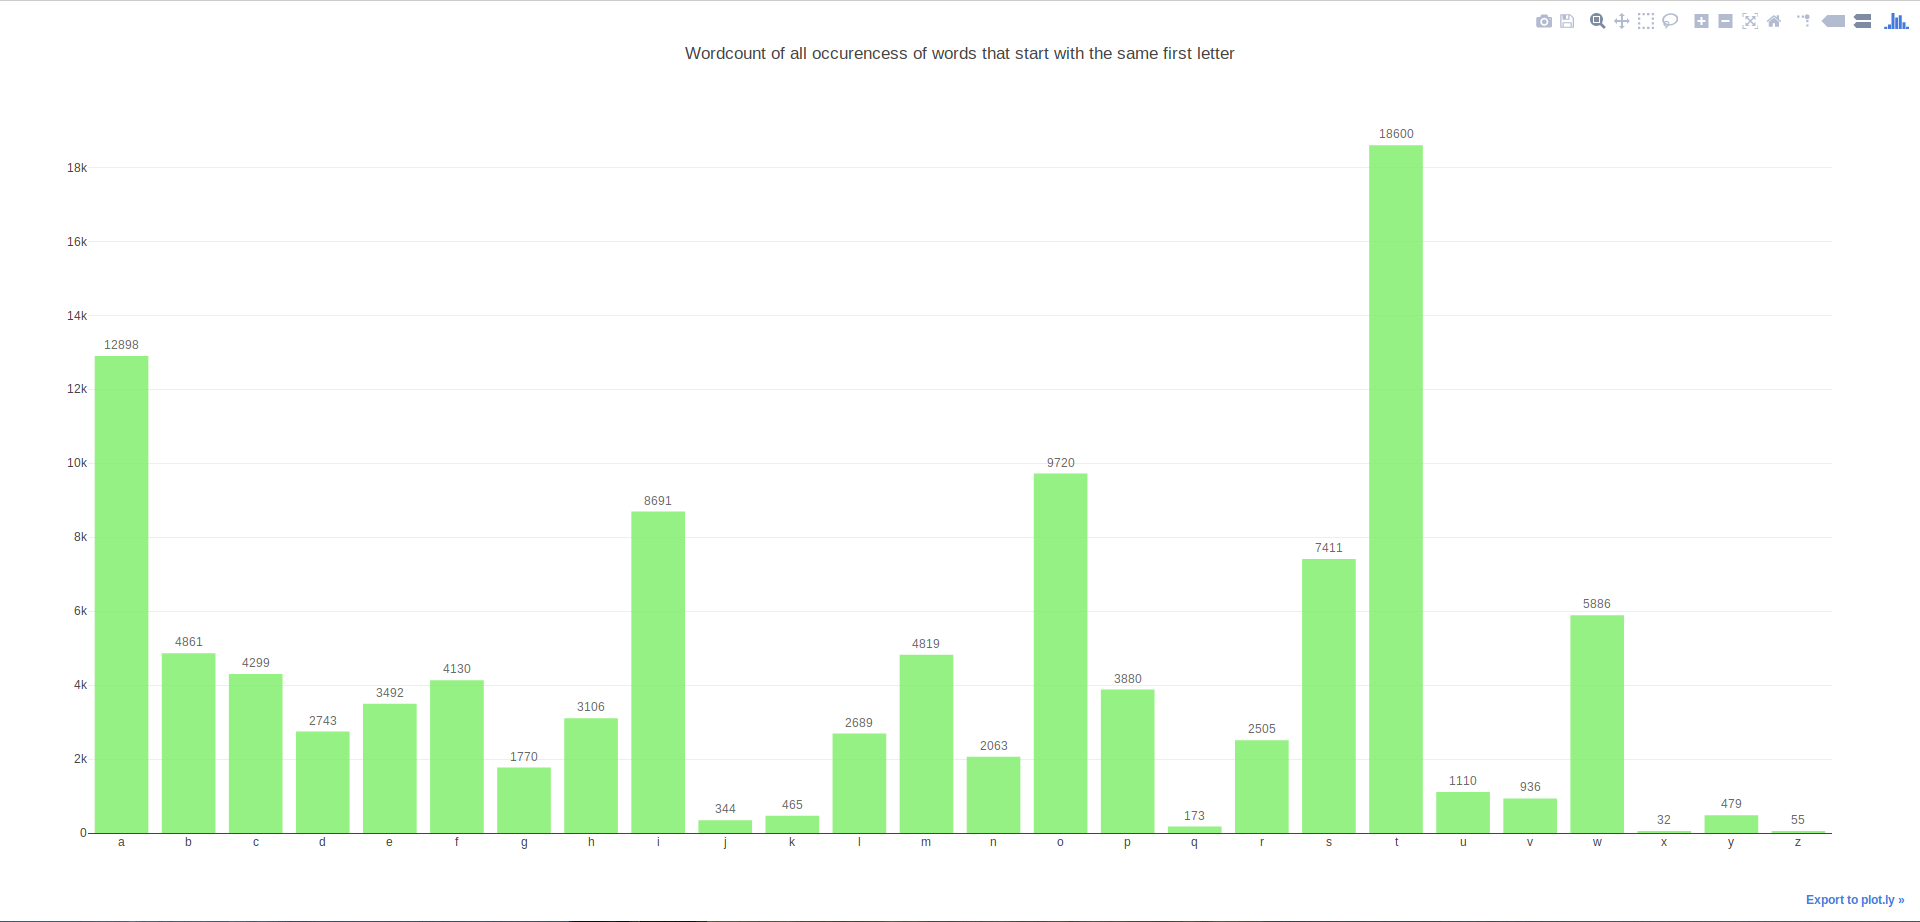
\includegraphics[scale=0.7]{Plots/Plot_Task_1_4.png}
    \caption{X-axis: Letters, Y-axis: Count, Scale: 1K}
    \label{fig:WordCount of letters}
	\end{figure}
\begin{figure}
    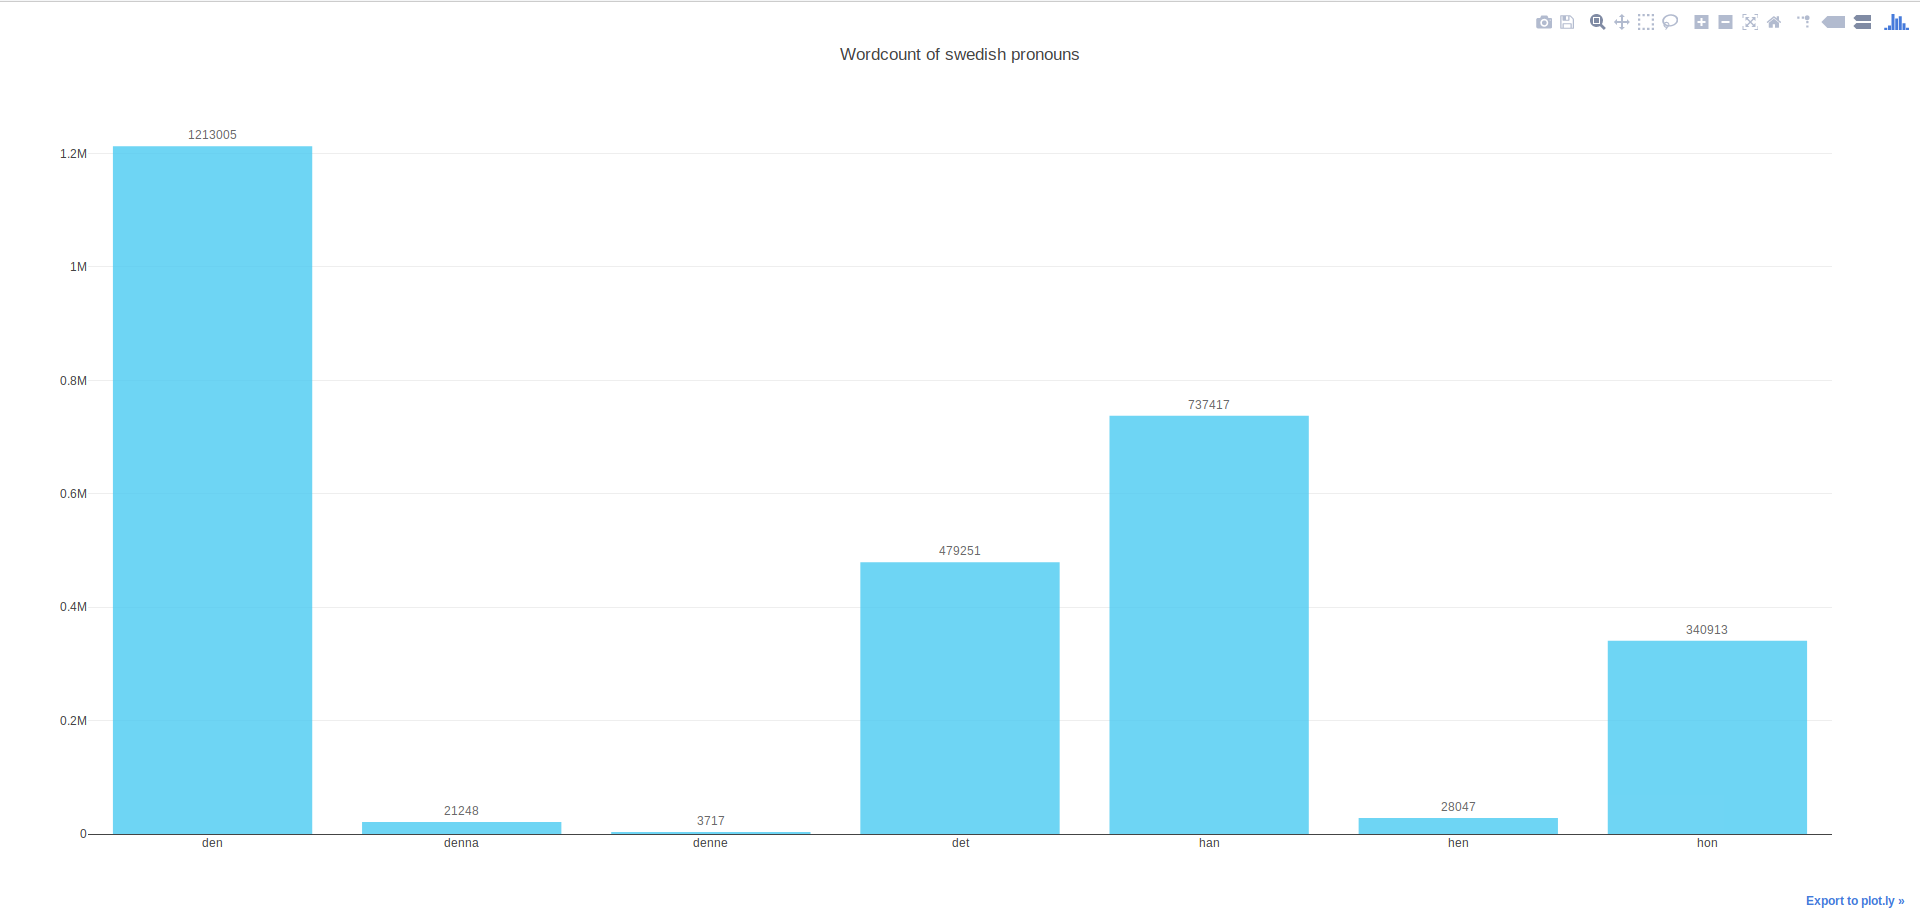
\includegraphics[scale=0.8]{Plots/Plot_Task_2.png}
    \caption{X-axis: Swedish Pronouns, Y-axis: Count, Scale: 1M}
    \label{fig:WordCount of pronouns}
	\end{figure}
\end{enumerate}
\hrule
\newpage
%-------------------------
\bibliography{sources}
\bibliographystyle{IEEEtran}
\end{document}